\documentclass{article}
\usepackage{import}
\documentclass{article}
\usepackage[paper=letterpaper,margin=2cm]{geometry}
\usepackage[utf8]{inputenc}
\usepackage[russian]{babel}
\usepackage[]{graphicx}
\usepackage[usenames]{color}
\usepackage{colortbl}
\usepackage{geometry}
\usepackage{xcolor}
\usepackage{hyperref}
\usepackage{../../lib/latex/listings-rust}
\usepackage{fontspec}
\setmonofont{JetBrains Mono}[Contextuals=Alternate,Ligatures = TeX,]
\usepackage{listings}
\usepackage{keycommand}
\usepackage{caption}

\setmainfont[
  Ligatures=TeX,
  Extension=.otf,
  BoldFont=cmunbx,
  ItalicFont=cmunti,
  BoldItalicFont=cmunbi,
]{cmunrm}
\setsansfont[
  Ligatures=TeX,
  Extension=.otf,
  BoldFont=cmunsx,
  ItalicFont=cmunsi,
]{cmunss}

\geometry{
  a4paper,
  top=25mm,
  right=30mm,
  bottom=25mm,
  left=30mm
}

\hypersetup{
  colorlinks=true,
  linkcolor=blue!50!red,
  urlcolor=blue!70!black
}

\captionsetup[lstlisting]{
  font={tt},
}

% based on Atom One Light
\lstset{
  language=Java,
  frame=single,
  basicstyle=\ttfamily\color[HTML]{383a42},
  columns=fullflexible,
  breaklines=true,
  numbers=left,
  frame=tab,
  postbreak=\mbox{\textcolor{red}{$\hookrightarrow$}\space},
  extendedchars=false,
  showspaces=false,
  showstringspaces=false,
  identifierstyle=\ttfamily\color[HTML]{4078f2},
  commentstyle=\color[HTML]{a0a1a7},
  stringstyle=\color[HTML]{50a14f},
  keywordstyle=\color[HTML]{a626a4},
  numberstyle=\ttfamily\color[HTML]{2c91af},
  rulecolor=\color[HTML]{383a42}
}

\lstdefinelanguage{XML}
{
  morestring=[b]",
  morestring=[s]{>}{<},
  morecomment=[s]{<?}{?>},
}

\newcommand{\code}[1]{
  \lstset{title=#1}
  \lstinputlisting{#1}
}
\newkeycommand{\itmo}[variant=aboba, labn=aboba, discipline=aboba, group=aboba, student=aboba,teacher=aboba, year=2022]{
  \begin{titlepage}
    \begin{center}
      \section*{
        Федеральное государственное автономное образовательное учреждение\\ высшего образования\\
        «Национальный исследовательский университет ИТМО»\\
        Факультет Программной Инженерии и Компьютерной Техники \\
       }
      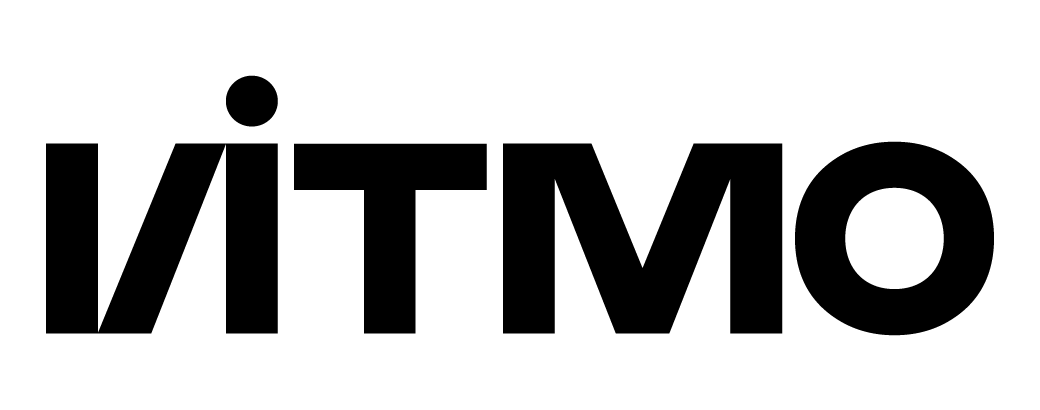
\includegraphics[scale=0.2]{../../lib/img/itmo.png}
    \end{center}

    \vspace{4cm}

    \begin{center}
      \large \textbf{Вариант \textnumero \commandkey{variant}}\\
      \textbf{Лабораторная работа \textnumero \commandkey{labn}}\\
      по дисциплине\\
      \textbf{\commandkey{discipline}}
    \end{center}

    \vspace*{\fill}

    \begin{flushright}
      Выполнил Студент группы \commandkey{group}\\
      \textbf{\commandkey{student}}\\
      Преподаватель: \\
      \textbf{\commandkey{teacher}}\\
    \end{flushright}

    \vspace{1cm}

    \begin{center}
      г. Санкт-Петербург\\
      \commandkey{year}г.
    \end{center}

    \thispagestyle{empty}
  \end{titlepage}
}



\begin{document}

\itmo[
  variant=371364,
  labn=3,
  discipline=Информационные системы и базы данных,
  group=P3115,
  student=Владимир Мацюк,
  teacher=Горбунов Михаил Витальевич,
  year=2023,
  logo=../../lib/img/itmo.png
]
\lstset{language=SQL}

\section{Текст задания}
Для отношений, полученных при построении предметной области из лабораторной работы №1, выполните следующие действия:
\begin{enumerate}
  \item Опишите функциональные зависимости для отношений полученной схемы (минимальное множество);
  \item Приведите отношения в 3NF (как минимум). Постройте схему на основеNF (как минимум).
  \item Опишите изменения в функциональных зависимостях, произошедшие после преобразования в 3NF (как минимум). Постройте схему на основеNF;
  \item Преобразуйте отношения в BCNF. Докажите, что полученные отношения представлены в BCNF. Если ваша схема находится уже в BCNF, докажите это;
  \item Какие денормализации будут полезны для вашей схемы? Приведите подробное описание.
  \item Придумайте триггер и связанную с ним функцию, относящиеся к вашей предметной области, согласуйте их с преподавателем и реализуйте на языке PL/pgSQL.
\end{enumerate}

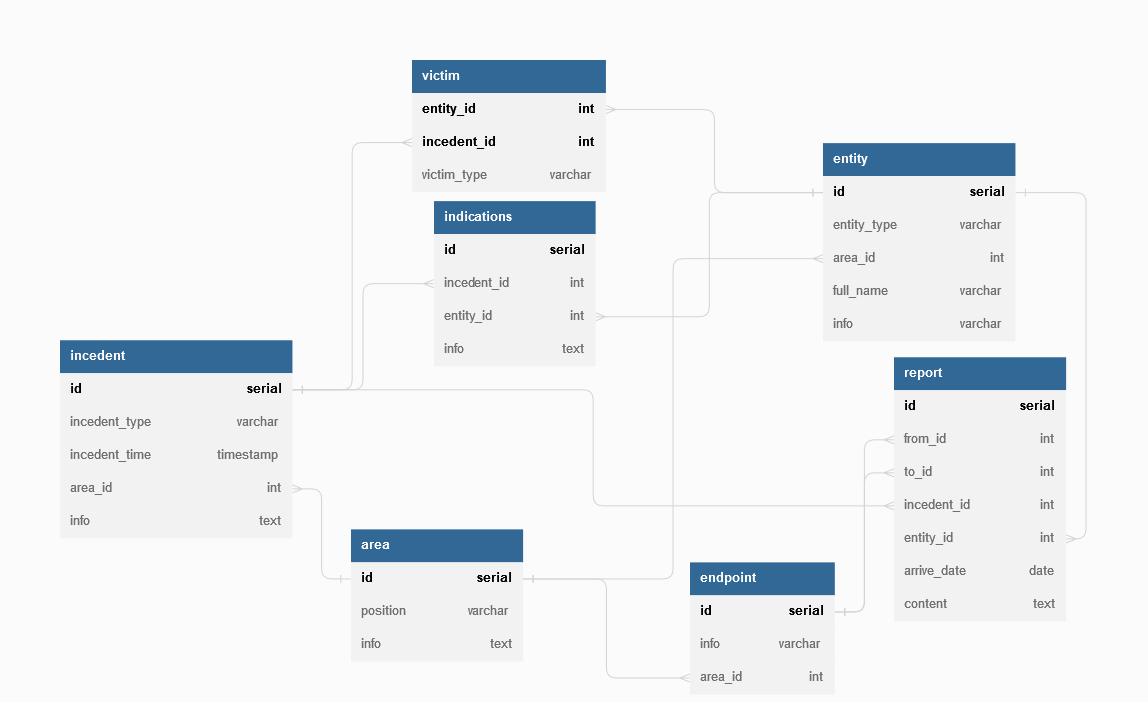
\includegraphics[width=\textwidth]{dbdiagram.png}

\section{Функциональные зависимости}
\begin{itemize} 
  \item area:    id -> (position, info);
  \item endpoint id -> (info, area\_id);
  \item entity: id -> (entity\_type, area\_id, full\_name, info);
  \item incedent: id -> (incedent\_type, incedent\_time, area\_id, info);
  \item report: id-> (from\_id, to\_id, incedent\_id, entity\_id, arrive\_date, content );
  \item indications: id -> (incedent\_id, entity\_id, info);
  \item victim:  (entity\_id, incedent\_id) -> (victim\_type)
\end{itemize}

\section{Нормальные формы}

\begin{itemize}
  \item 1NF: Моя модель удовлетворяет 1NF, так как все атрибуты атомарны, и нет повторяющихся групп.
        
  \item 2NF: Моя модель удовлетворяет 2NF, так как все неключевые атрибуты полностью функционально зависят от первичных ключей.
        
  \item 3NF: Моя модель удовлетворяет 3NF, так как все неключевые атрибуты зависят только от первичных ключей, и не содержат транзитивных зависимостей.
        
\end{itemize}
\section{BCNF}
Моя модель удовлетворяет BCNF, так как для все части составного первичного ключа не зависят от неключевого столбца.

\section{Денормализация}

\begin{itemize}
  \item Добавление избыточных атрибутов: В некоторых случаях добавление избыточных атрибутов может улучшить производительность запросов. Например, если часто запрашивается отправная и точка назначения в репорте, можно добавить атрибут from\_postition и to\_postition в таблицу report. Это позволит избежать дополнительных запросов или операци JOIN при каждом запросе, однако необходимо будет обновлять этот атрибут при добавлении или изменении таблиц area и endpoint.
        
  \item Объединение связанных таблиц: В некоторых случаях, объединение таблиц может уменьшить количество операций JOIN и ускорить обработку запросов. Например, можно рассмотреть объединение таблиц area и endpoint, если часто запрашиваются данные о местности и конечной точки одновременно.
\end{itemize}


\section{Функция на языке PL/pgSQL}

Функция всавляет текущую дату в таблицу report, усли она не была указана.
\code{trigger.psql}

\section{Вывод}
При выполнении лабораторной работы я познакомился с понятием нормализации и денормализации. Научился определять функциональные зависимости модели, а также анализировать последнюю на соответствие различным нормальным формам. Познакомился с процедурным языком PL/pgSQL. Изучил эффективные способы денормализации схемы базы данных и ситуации, в которых возможно их применение.

\end{document}
